%--------------------------------------------
% Chapter: RASPBERRY PI BASED HARDWARE PLATFORM
%--------------------------------------------
\chapter{Raspberry Pi based hardware platform}
\label{sec:hardware}
%- - - - - - - - - - - - - - - - - - - - - - 
% Section: Basic components and sensors
%- - - - - - - - - - - - - - - - - - - - - - 
\section{Hardware and device communication}
\label{sec:hardware:Hardware}

%- - - - - - - - - - - - - - - - - - - - - - 
% Subsection: Basic components and sensors
%- - - - - - - - - - - - - - - - - - - - - - 
\subsection{Basic components and chosen sensors}
\label{sec:hardware:Components}

As the main computing board the Raspberry Pi B+ has been chosen. At time of start of this project, there has been no stable Real-Time Kernel Patch (PREEMPT\_RT) for the multi-core CPU Broadcom BCM2709 of Raspberry Pi 2. Fortunately, the 40-pin expansion breakout of Raspberry Pi A+/B+ and Raspberry Pi 2 are identical. In consequence, all the chosen peripheral hardware and sensors are compatible with Raspberry Pi 2. In future projects, it should be a minor task to update the Kernel of the pre-configured OS Image delivered in this project and make a Raspberry Pi 2 running with this platform. A complete list of all components with pictures can be found in chapter \ref{sec:hardware:BillOfMat}.

The main components chosen for this project are:
\begin{itemize}
	\item \textbf{Main board:}\\
	\texttt{Raspberry Pi A+/B+} in this project. In future projects, also the \texttt{Raspberry Pi 2} is compatible with the chosen hardware as soon as a Raspberry Pi 2 compatible PREEMPT\_RT Kernel Patch is available.
	
	\item \textbf{Expansion Board:}\\
	\texttt{Adafruit GPS Hat}, including a \texttt{GlobalTop GPS} receiver with builtin Chip-Antenna. The GPS is connected via UART to the Raspberry Pi board. In consquence, the UART may not be used for other purposes and is blocked when the GPS Hat is assembled to the Raspberry Pi!
	
	\item \textbf{Inertial Measurement Unit (IMU):}\\
	\texttt{Polulu AltiIMU v4 (10-DOF version)}. The Inertial Measurement Unit comprises sensors that enables to measure the pose of the Quadrocopter in space. Rotational speed, acceleration rates for each axis in space and the barometric air pressure can be sensed with the chosen IMU. The IMU is connected via I2C to the Raspberry Pi board.
	
	In consequence, the following sensors are included in the chosen IMU:
	\begin{itemize}
		\item \textbf{3D Accelerometer:} \texttt{ST LSM303D} (including 3D Magnetometer/e-Compass)
		\item \textbf{3D MEMS Gyroscope:} \texttt{ST L3GD20H}
		\item \textbf{3D Magnetometer:} \texttt{ST LSM303D} (including 3D Accelerometer)
		\item \textbf{Absolute MEMS Barometer:} \texttt{ST LPS331AP}
	\end{itemize}
	
	\item \textbf{A/D Converter:}\\
	\texttt{Adafruit ADS1015} including ADC Chip \texttt{Texas Instruments ADS1015}. The ADC breakout board is connected via I2C to the Raspberry Pi board.
	
	\item \textbf{DC/DC Power converter:}\\
	\texttt{Polulu D15V70F5S3}. Since the Raspberry Pi board including all peripherals is aimed to be connected to the Li-Ion battery of the HElikopter Quadrocopters of Hochschule Esslingen, a separate DC/DC power converter has been included to the controller platform. The power converter ensures a stable power supply voltage of 5V DC at a continuous current draw up to 3.5A.
\end{itemize}

%- - - - - - - - - - - - - - - - - - - - - - 
% Subsection: I2C Adressing
%- - - - - - - - - - - - - - - - - - - - - - 
\subsection{I2C adressing}
\label{sec:hardware:Components:Adressing}

This section shows all necessary transmissions which are needed for a successful interfacing on the I$^2$C bus. 

\begin{itemize}
	\item \subsubsection{\underline{\textbf{A/D Converter}}}
\label{sec:hardware:Components:Adressing:ADC}

%\textbf{I$^2$C slave adress:\\
\textbf{I$^2$C slave address}: \texttt{0b1001001 (0x49)}

\subsubsection{Read}
\label{subsec:ADCread}

The read command get's the data from the address, which is stored in the pointer register (blue color). See figure \ref{fig:ADC1}

\begin{figure}[H]
	\centering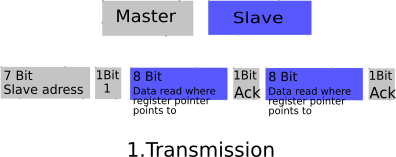
\includegraphics[width=0.7\textwidth]{fig/I2C_Adressing/ADC_read}
	\caption{Scheme to read data from the ADC}
	\label{fig:ADC1}
\end{figure}

\subsubsection{Write}
\label{subsec:ADCwrite}


\begin{figure}[H]
	\centering\includegraphics[width=0.7\textwidth]{fig/I2C_Adressing/ADC_write}
	\caption{Scheme to write data to the ADC}
	\label{fig:ADC2}
\end{figure}

\subsubsection{Read conversion register}
\label{subsec:ADCconversion}
To enable a read from a conversion register, several packages need to be sent. They can be seen in figure \ref{fig:ADC3}. All slave and master acknowledges are not shown because they are handled direct by the interface and so not important for the application.

\begin{figure}[H]
	\centering\includegraphics[width=0.9\textwidth]{fig/I2C_Adressing/ADC_read_conversion}
	\caption[Scheme to read the ADC's conversion registers]{Transmission scheme to read the ADC's conversion registers}
	\label{fig:ADC3}
\end{figure}

\item \subsubsection{\underline{\textbf{Inertial Measurement Unit (IMU)}}}
\label{sec:hardware:Components:Adressing:IMU}

The Inertial measurement unit (IMU) has three different chips mounted. Each chip solves one of the measurements of this unit. Each chip has a different I$^2$C address. All slave and master acknowledges are not shown because they are handled direct by the interface and are not important to the application level.
 \begin{itemize}
	 \item \subsubsection*{\underline{\textbf{Acceleration and Magnet Sensor}}}
\label{sec:hardware:Components:Adressing:IMU:ACC}

\textbf{I$^2$C slave address}: \texttt{0b0011110 (0x1E)}

There are several registers which have to be configured before reading and also several register where the acceleration, magnetic strength and if needed temperature can be read. To reduce the amount of pages of this document, they will be not listed here. All the registers can be found in the datasheet \texttt{IMU\_LSM303D.pdf}, stored in the SVN directory \texttt{/doc/se/Datasheets/IMU}.


\subsubsection{Read}
\label{subsubsec:ACCread}

\begin{figure}[H]
	\centering\includegraphics[width=0.7\textwidth]{fig/I2C_Adressing/ACC_read_single}
	\caption{Transmission scheme for a single byte read of the ACC-Sensor}
	\label{fig:ACC1}
\end{figure}

\begin{figure}[H]
	\centering\includegraphics[width=0.8\textwidth]{fig/I2C_Adressing/ACC_read_multiple}
	\caption[Scheme for multiple data read of the ACC-Sensor]{Transmission scheme for multiple data read of the ACC-Sensor(burst read)}
	\label{fig:ACC2}
\end{figure}

\textbf{1. Transmission}: Slave address including RW bit ('0'): \texttt{0x3C}\\
\textbf{2. Transmission}: Slave address including RW bit ('1'): \texttt{0x3D}

\subsubsection{Write}
\label{subsubsec:ACCwrite}

\begin{figure}[H]
	\centering\includegraphics[width=0.55\textwidth]{fig/I2C_Adressing/ACC_write_single}
	\caption[Scheme for a single byte write of the ACC-Sensor]{Transmission scheme for a single byte write of the ACC-Sensor}
	\label{fig:ACC3}
\end{figure}

\begin{figure}[H]
	\centering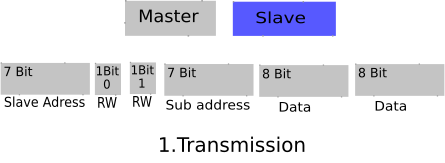
\includegraphics[width=0.7\textwidth]{fig/I2C_Adressing/ACC_write_multiple}
	\caption[Scheme for multiple data write of the ACC-Sensor]{Transmission scheme for multiple data write of the ACC-Sensor(burst write)}
	\label{fig:ACC4}
\end{figure}

\textbf{1.Transmission}: Slave address including RW bit ('0'): \texttt{0x3C}


\item \subsubsection*{\underline{\textbf{Gyroscope Sensor}}}
\label{sec:hardware:Components:Adressing:IMU:Gyro}

\textbf{I$^2$C slave address}: \texttt{0b1101010 (0x6A)}

There are several registers which have to be configured before reading and also several register where the rotational speed and if needed the temperature can be read. To reduce the amount of pages of this document, they will be not listed here. All the registers can be found in the datasheet \texttt{IMU\_L3GD20H.pdf}, which is stored in the SVN directory \texttt{\textbackslash{}doc\textbackslash{}se\textbackslash{}Datasheets\textbackslash{}IMU}.

\subsubsection{Read}
\label{subsubsec:Gyroread}

\begin{figure}[H]
	\centering\includegraphics[width=0.7\textwidth]{fig/I2C_Adressing/ACC_read_single}
	\caption{Transmission scheme for a single byte read of the Gyro-Sensor}
	\label{fig:Gyro1}
\end{figure}

\begin{figure}[H]
	\centering\includegraphics[width=0.8\textwidth]{fig/I2C_Adressing/ACC_read_multiple}
	\caption[Scheme for multiple data read of the Gyro-Sensor]{Transmission scheme for multiple data read of the Gyro-Sensor (burst read)}
	\label{fig:Gyro2}
\end{figure}

\textbf{1.Transmission}: Slave address including RW bit ('0'): \texttt{0xD4}\\
\textbf{2.Transmission}: Slave address including RW bit ('1'): \texttt{0xD5}

\subsubsection{Write}
\label{subsubsec:Gyrowrite}

\begin{figure}[H]
	\centering\includegraphics[width=0.55\textwidth]{fig/I2C_Adressing/ACC_write_single}
	\caption[Scheme for a single byte write of the Gyro-Sensor]{Transmission scheme for a single byte write of the Gyro-Sensor}
	\label{fig:Gyro3}
\end{figure}

\begin{figure}[H]
	\centering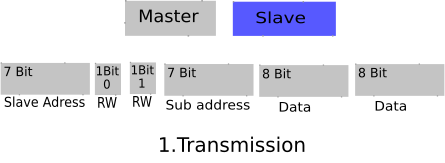
\includegraphics[width=0.7\textwidth]{fig/I2C_Adressing/ACC_write_multiple}
	\caption[Scheme for multiple data write of the Gyro-Sensor]{Transmission scheme for multiple data write of the Gyro-Sensor (burst write)}
	\label{fig:Gyro4}
\end{figure}

\textbf{1.Transmission}: Slave address including RW bit ('0'): \texttt{0xD4}

\item \subsubsection*{\underline{\textbf{Pressure Sensor}}}
\label{sec:hardware:Components:Adressing:IMU:Pressure}

\textbf{I$^2$C slave address}: \texttt{0b1011100 (0x5C)}

There are several registers which have to be configured before reading and also several register where the pressure and if needed the temperature can be read. To reduce the amount of pages of this document, they will be not listed here. All the registers can be found in the datasheet \texttt{IMU\_LPS331AP.pdf}, which is stored in the SVN directory \texttt{\textbackslash{}doc\textbackslash{}se\textbackslash{}Datasheets\textbackslash{}IMU}.

\subsubsection{Read}
\label{subsubsec:Pressureread}

\begin{figure}[H]
	\centering\includegraphics[width=0.7\textwidth]{fig/I2C_Adressing/ACC_read_single}
	\caption[Scheme for a single byte read of the Pressure-Sensor]{Transmission scheme for a single byte read of the Pressure-Sensor}
	\label{fig:Pressure1}
\end{figure}

\begin{figure}[H]
	\centering\includegraphics[width=0.80\textwidth]{fig/I2C_Adressing/ACC_read_multiple}
	\caption[Scheme for multiple data read of the Pressure-Sensor]{Transmission scheme for multiple data read of the Pressure-Sensor(burst read)}
	\label{fig:Pressure2}
\end{figure}

\textbf{1.Transmission}: Slave address including RW bit ('0'): \texttt{0xB8}\\
\textbf{2.Transmission}: Slave address including RW bit ('1'): \texttt{0xB9}

\subsubsection{Write}
\label{subsubsec:Pressurewrite}

\begin{figure}[H]
	\centering\includegraphics[width=0.55\textwidth]{fig/I2C_Adressing/ACC_write_single}
	\caption[Scheme for a single byte write of the Pressure-Sensor]{Transmission scheme for a single byte write of the Pressure-Sensor}
	\label{fig:Pressure3}
\end{figure}

\begin{figure}[H]
	\centering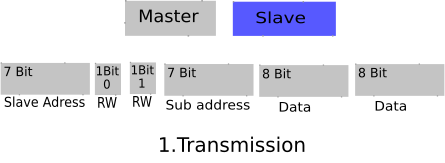
\includegraphics[width=0.7\textwidth]{fig/I2C_Adressing/ACC_write_multiple}
	\caption[Scheme for multiple data write of the Pressure-Sensor]{Transmission scheme for multiple data write of the Pressure-Sensor(burst write)}
	\label{fig:Pressure4}
\end{figure}

\textbf{1.Transmission: Slave address including RW bit ('0'): 0xB8}
\end{itemize}

\item \subsubsection{\underline{\textbf{Motor Driver}}}
\label{sec:hardware:Components:Adressing:IMU:ADC}

All slave and master acknowledges are not shown because they are handled direct by the interface and so not important here. To enable flying with a Quadrocopter there are four motors and so four brushless drivers needed. Each of them has an individual address.

\pagebreak[3]{
\textbf{I$^2$C slave addresses}:\\
Motor 1  --> \texttt{0b0101001 (0x29)}\\
Motor 2  --> \texttt{0b0101010 (0x2A)}\\
Motor 3  --> \texttt{0b0101011 (0x2B)}\\
Motor 4  --> \texttt{0b0101100 (0x2C)}}

\subsection{Read}
\label{subsec:Motorread}

\textbf{Read operations}: NOT DEFINED	

\subsection{Write}
\label{subsec:Motorwrite}

\textbf{Write operations}:

Possible data values are in the range of \texttt{10} (Decimal) up to \texttt{255} (Decimal) which refers to a hexadecimal range of \texttt{0x0A} to \texttt{0xFF}.

\begin{figure}[H]
	\centering\includegraphics[width=0.4\textwidth]{fig/I2C_Adressing/Motor_write}
	\caption[Scheme for a single byte write to a motor driver board]{Transmission scheme for a single byte write to a motor driver board}
	\label{fig:Motor}
\end{figure}


\pagebreak[3]{
\textbf{1.Transmission}: Slave address including RW bit ('0'):\\
Motor 1 --> \texttt{0x52}\\
Motor 2 --> \texttt{0x54}\\
Motor 3 --> \texttt{0x56}\\
Motor 4 --> \texttt{0x58}}

\textbf{Possible Data values are in the range of 10 (Decimal) up to 255 (Decimal). So in the range from 0x0A to 0xFF.}

\end{itemize}

%- - - - - - - - - - - - - - - - - - - - - - 
% Section: UART communication
%- - - - - - - - - - - - - - - - - - - - - - 
\subsection{UART communication}
\label{sec:hardware:Components:UART}
The GPS module uses the UART interface of the Raspberry Pi. The used GPS module has a fixed communication set up.\\
To ensure working the following values need to be used:
\begin{itemize}
	\item Baudrate: 9600 baud
	\item Databits: 8 Bits
	\item Stopbits:	1 Bit
	\item Modem control: No
\end{itemize}


%- - - - - - - - - - - - - - - - - - - - - - 
% Section: Technical drawings and packaging
%- - - - - - - - - - - - - - - - - - - - - - 
\section{Technical drawings and packaging}
\label{sec:hardware:techDrawAndPack}

\begin{figure}[H]
    \centering
    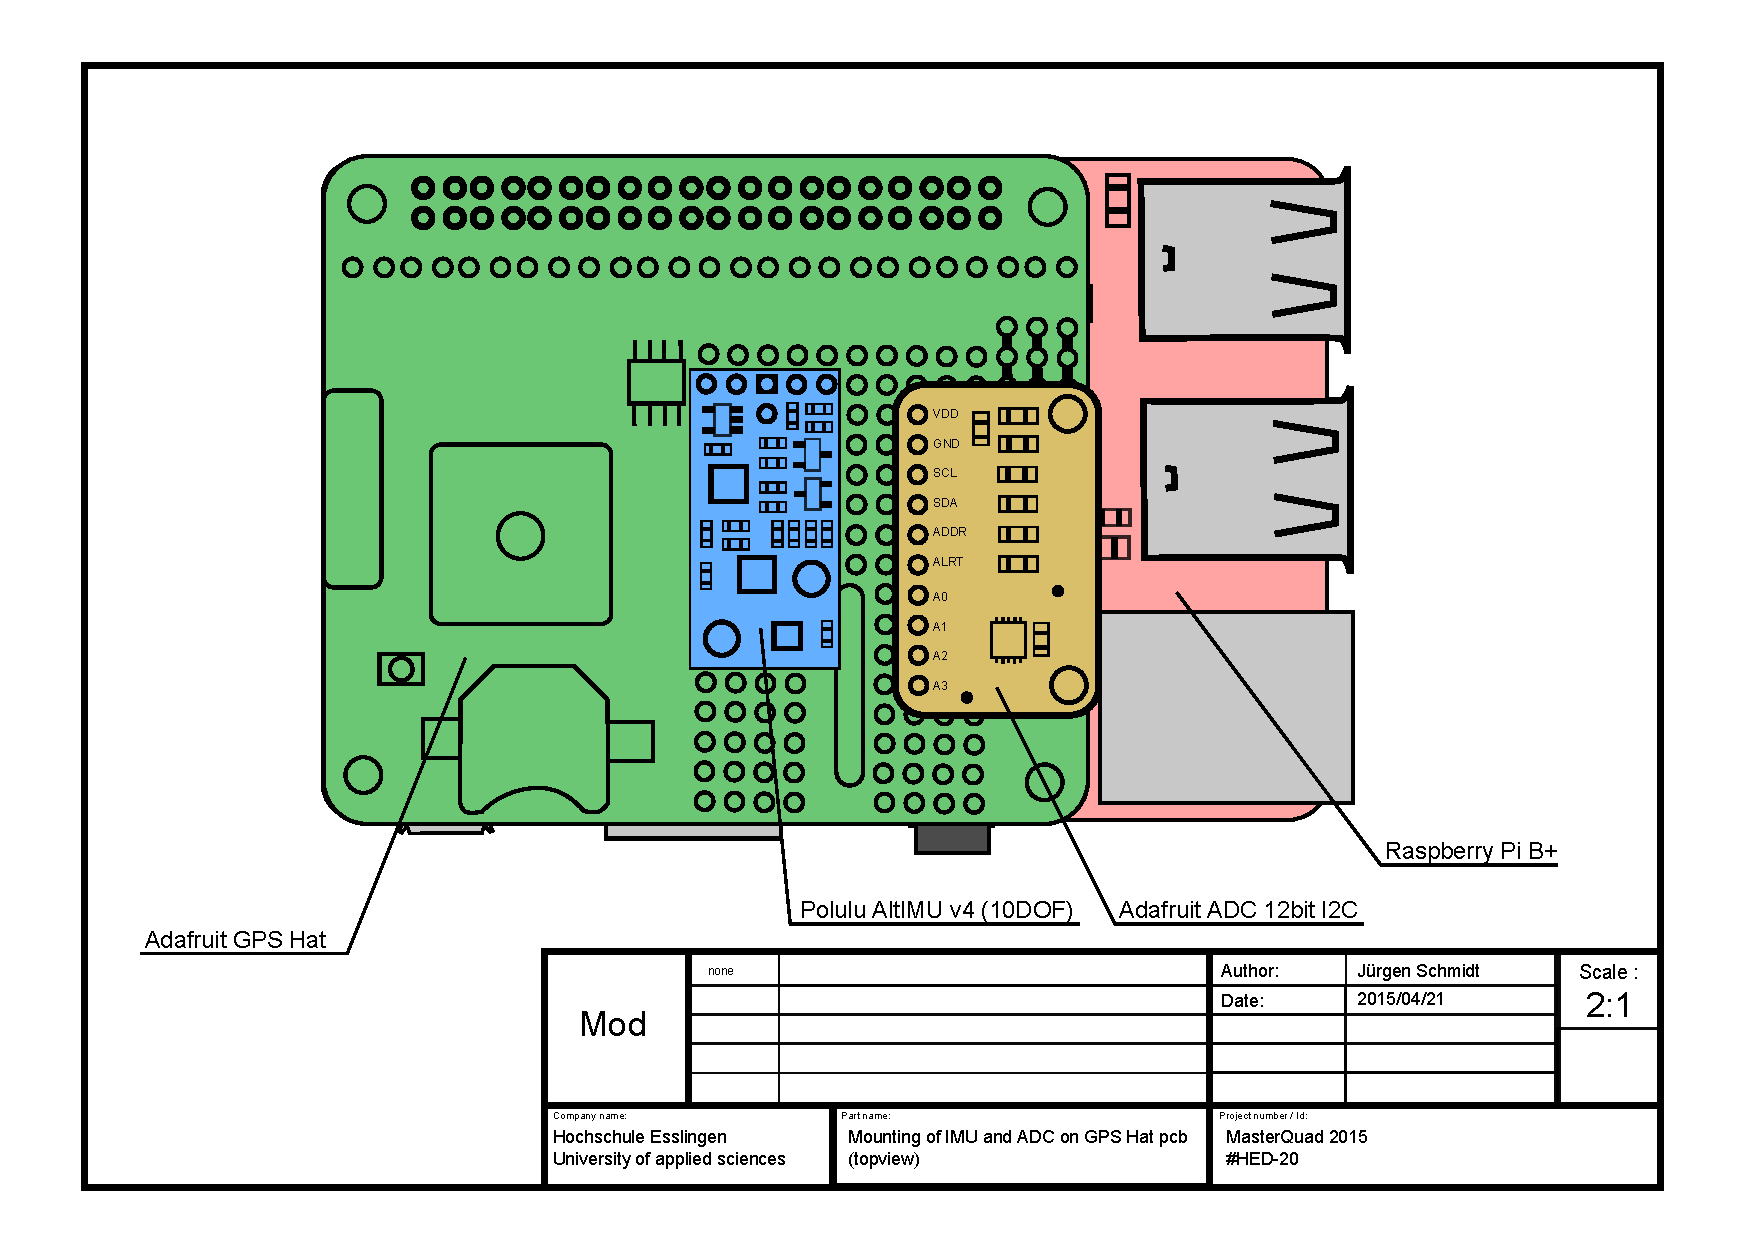
\includegraphics[angle=90,width=0.83\textwidth]{fig/ch-rpi-hardware/A4_tech_draw_topview_sensor_mountingPositions}
    \caption[Placing ADC and IMU on GPS Hat]{Placing ADC and IMU on GPS Hat. The drawing shows the exact position of the sensor boards, aligned with matching soldering pads of the GPS Hat and the Sensor baords.}
    \label{fig:hardware:sensorMount}
\end{figure}

To mount the assembled GPS Hat on top of the Raspberry Pi (as depicted in fig. \ref{fig:hardware:stackedMount}) the following parts are required:
\begin{itemize}
	\item 4 pcs. polyamid standoffs, 10mm height (B\"urklin, 18H5045)
	\item 4 pcs. threaded rod, M2.5 in 40mm pieces (B\"urklin, 16H322)
	\item 16 pcs. polyamid shims, M2.5 (B\"urklin, 16H942)
	\item 12 pcs. hexagonal nuts, M2.5 (B\"urklin, 16H722)
	\item 1 pc. GPS Hat with assembled sensors/peripherals as shown in fig. \ref{fig:hardware:sensorMount} and soldered according to \ref{fig:hardware:soldering:top} and fig. \ref{fig:hardware:soldering:bottom}
	\item 1 pc. Raspberry Pi A+/B+/2
\end{itemize}
All referenced parts are also mentioned in the Bill of Materials in Chapter \ref{sec:hardware:BillOfMat}.

\begin{figure}[H]
    \centering
    \includegraphics[width=0.87\textwidth]{fig/ch-rpi-hardware/A4_tech_draw_sideview_stackedMount}
    \caption{Stacked mounting of Hat-Board on Raspberry Pi}
    \label{fig:hardware:stackedMount}
\end{figure}

To ease the soldering of the IMU and ADC on top of the GPS Hat board, a soldering layout has been created as shown in fig. \ref{fig:hardware:soldering:top} and fig. \ref{fig:hardware:soldering:bottom}. The layout shows in a one-by-one view the soldering pads of the GPS Hat (one view onto the top, one view onto the bottom). According to the experience of the authors of this document, the soldering layout figures eases the soldering of the sensors to the GPS Hat for students, that are not used to solder a densely packed PCB.

\begin{figure}[H]
    \centering
    \includegraphics[width=0.87\textwidth]{fig/ch-rpi-hardware/A4_tech_draw_topview_gpshat_soldering}
    \caption{Soldering plan for Raspberry Pi Hat (top view)}
    \label{fig:hardware:soldering:top}
\end{figure}

\begin{figure}[H]
    \centering
    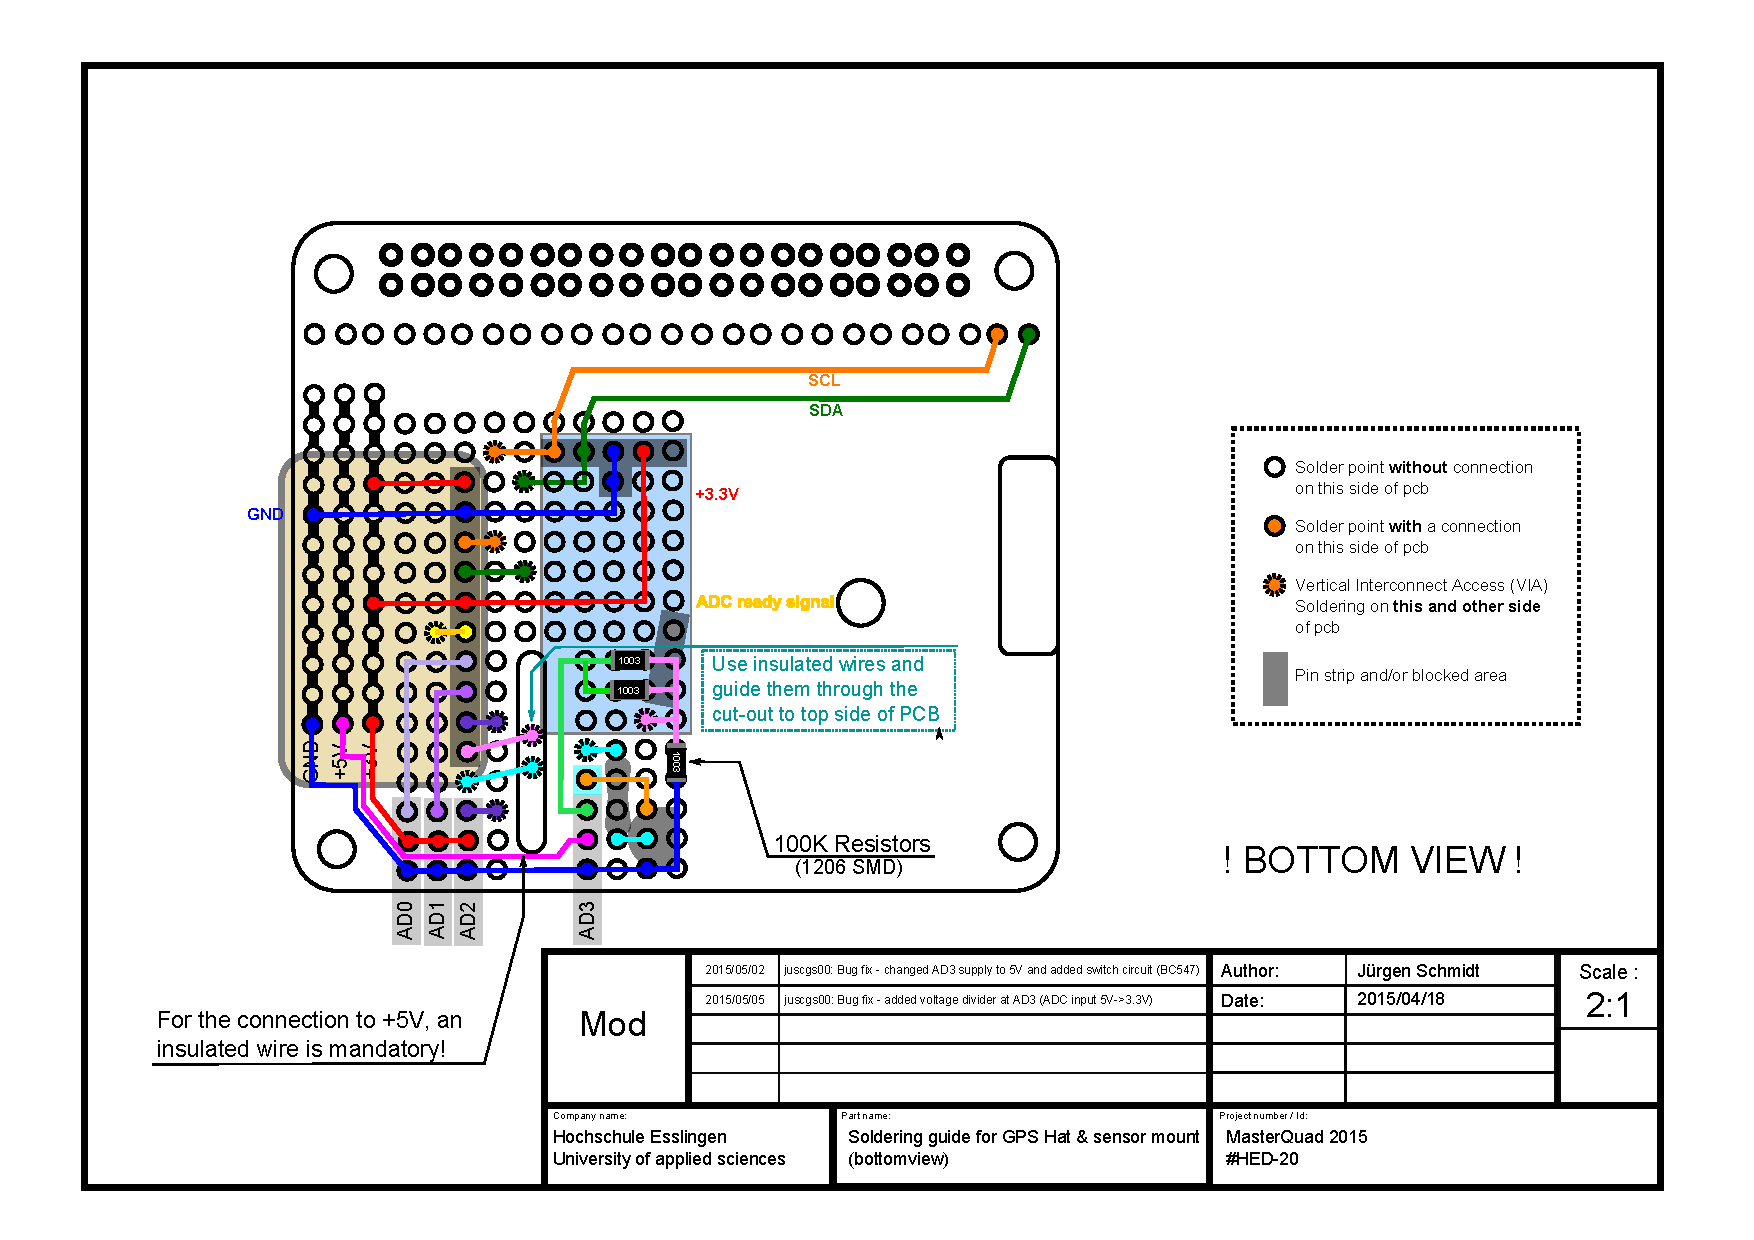
\includegraphics[width=0.87\textwidth]{fig/ch-rpi-hardware/A4_tech_draw_bottomview_gpshat_soldering}
    \caption{Soldering plan for Raspberry Pi Hat (bottom view)}
    \label{fig:hardware:soldering:bottom}
\end{figure}

\begin{figure}[H]
    \centering
    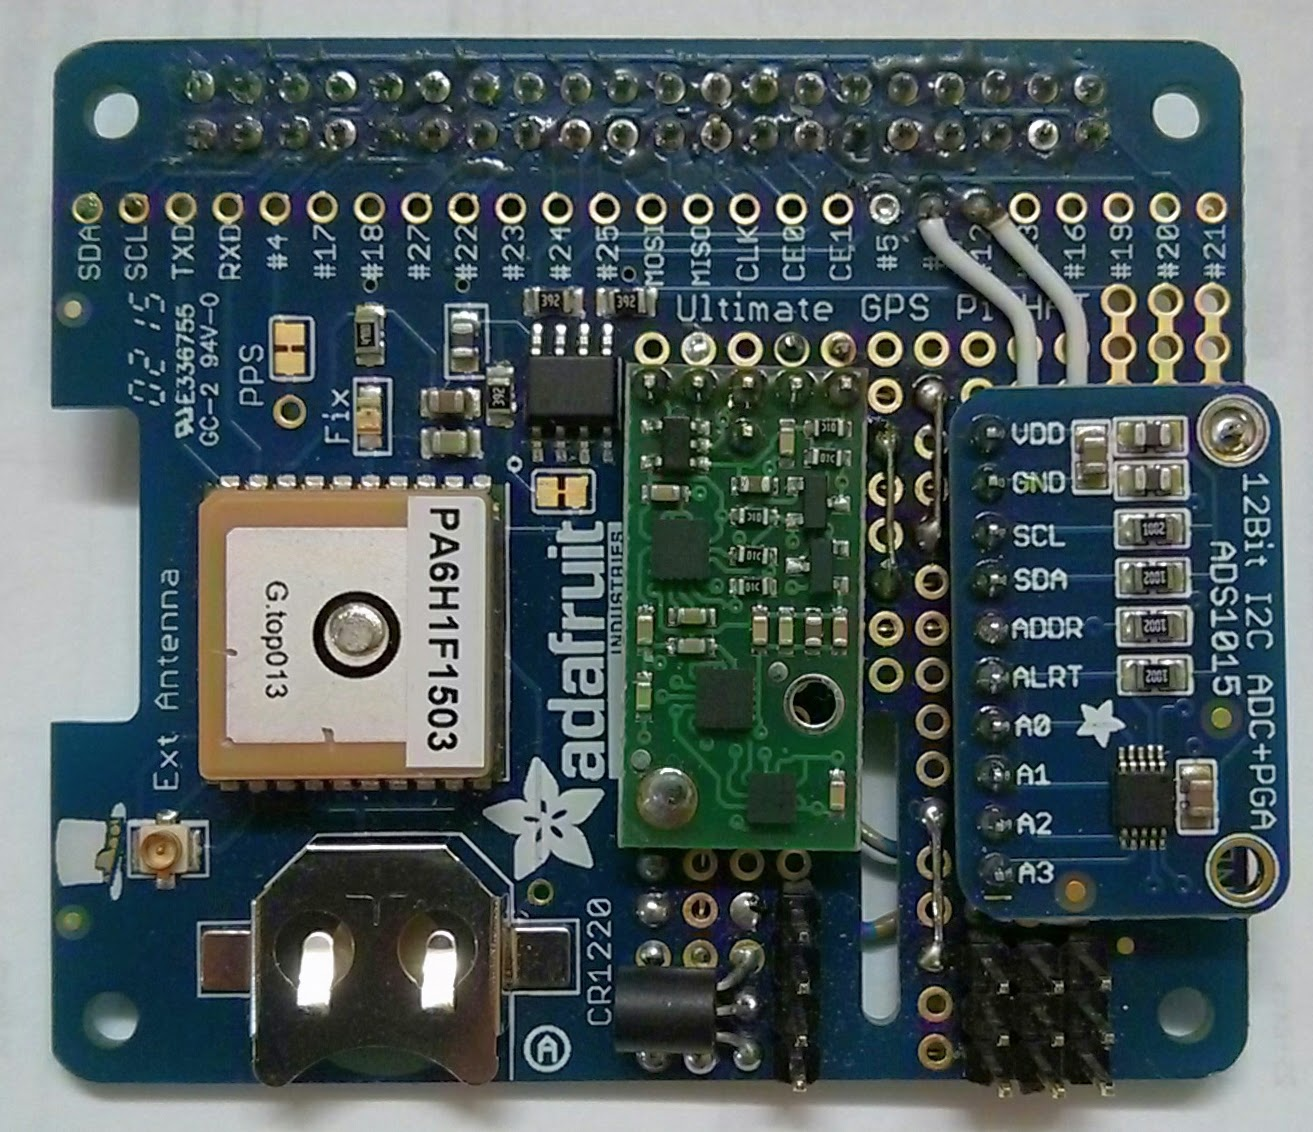
\includegraphics[width=0.71\textwidth]{fig/ch-rpi-hardware/picHatTop}
    \caption{Soldered Raspberry Pi Hat (top view)}
    \label{fig:hardware:mountedHat:top}
\end{figure}

\begin{figure}[H]
    \centering
    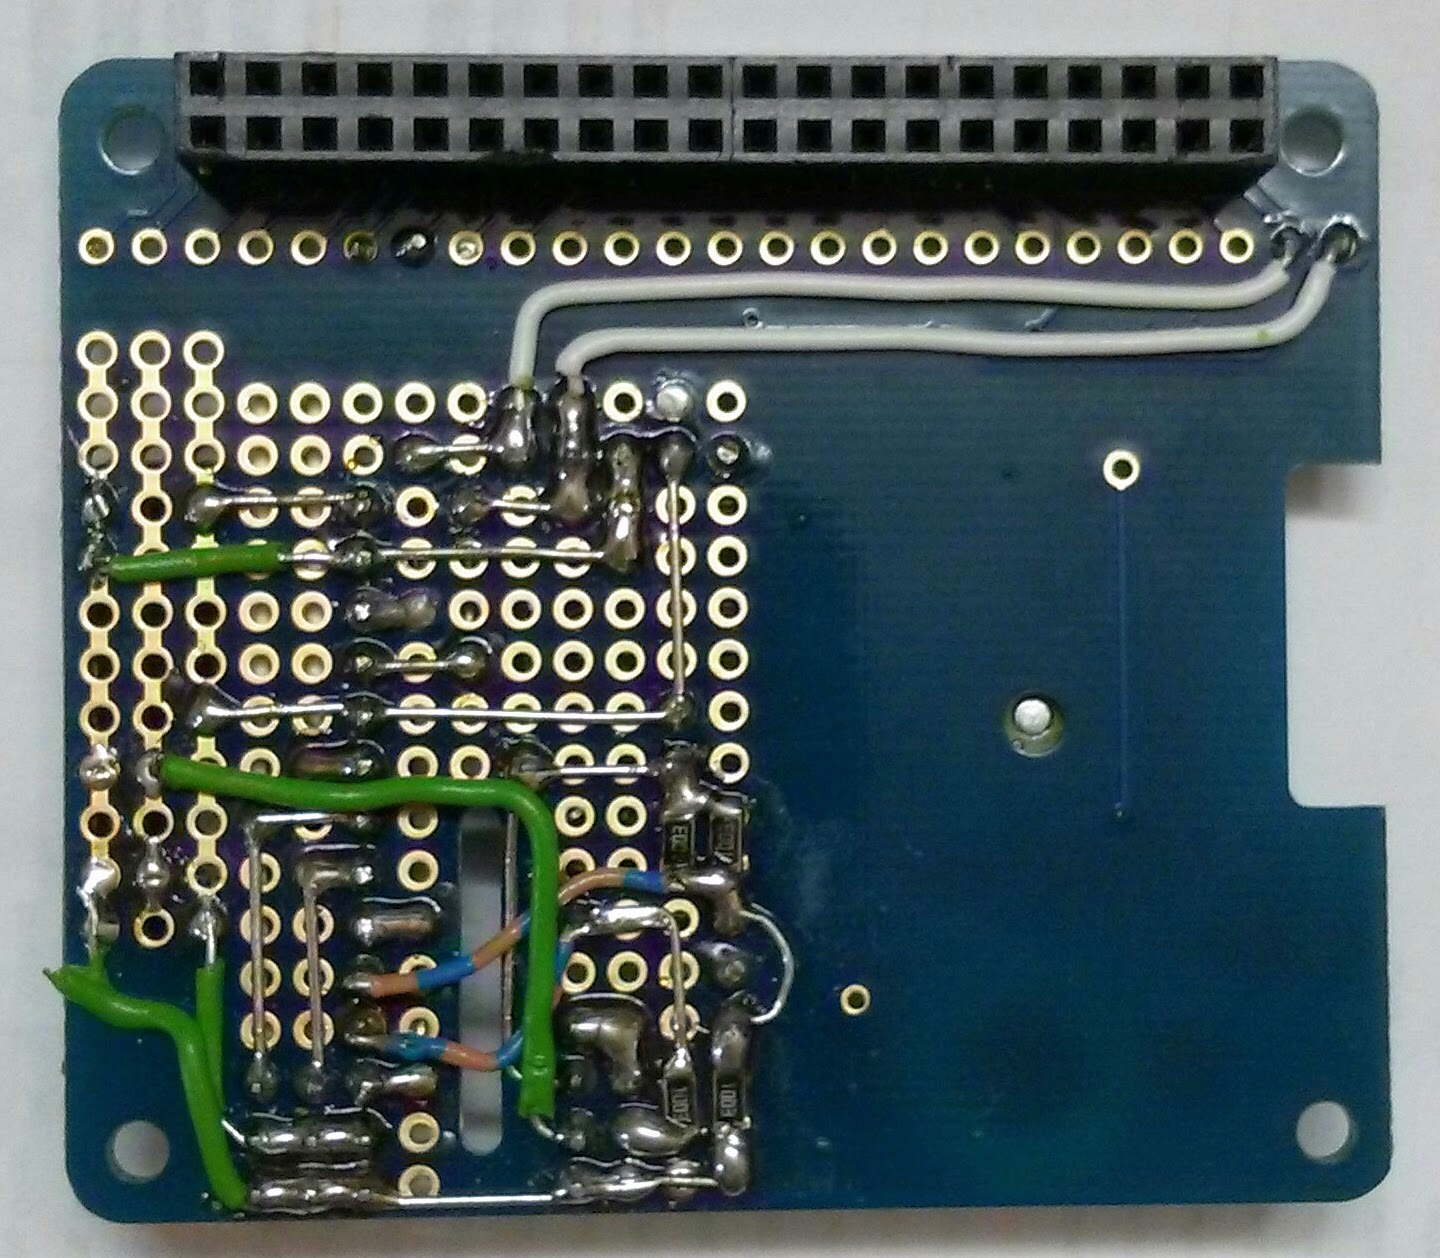
\includegraphics[width=0.71\textwidth]{fig/ch-rpi-hardware/picHatBottom}
    \caption{Soldered Raspberry Pi Hat (bottom view)}
    \label{fig:hardware:mountedHat:bottom}
\end{figure}

%- - - - - - - - - - - - - - - - - - - - - - 
% Section: Bill of materials
%- - - - - - - - - - - - - - - - - - - - - - 
\newpage
\section{Bill of materials}
\label{sec:hardware:BillOfMat}

For this project, the parts nedded for the Raspberry Pi Platform has been ordered 5 times. The following Bill of Materials lists all parts including the distributor and parts numbers.

\begin{figure}[H]
    \centering
    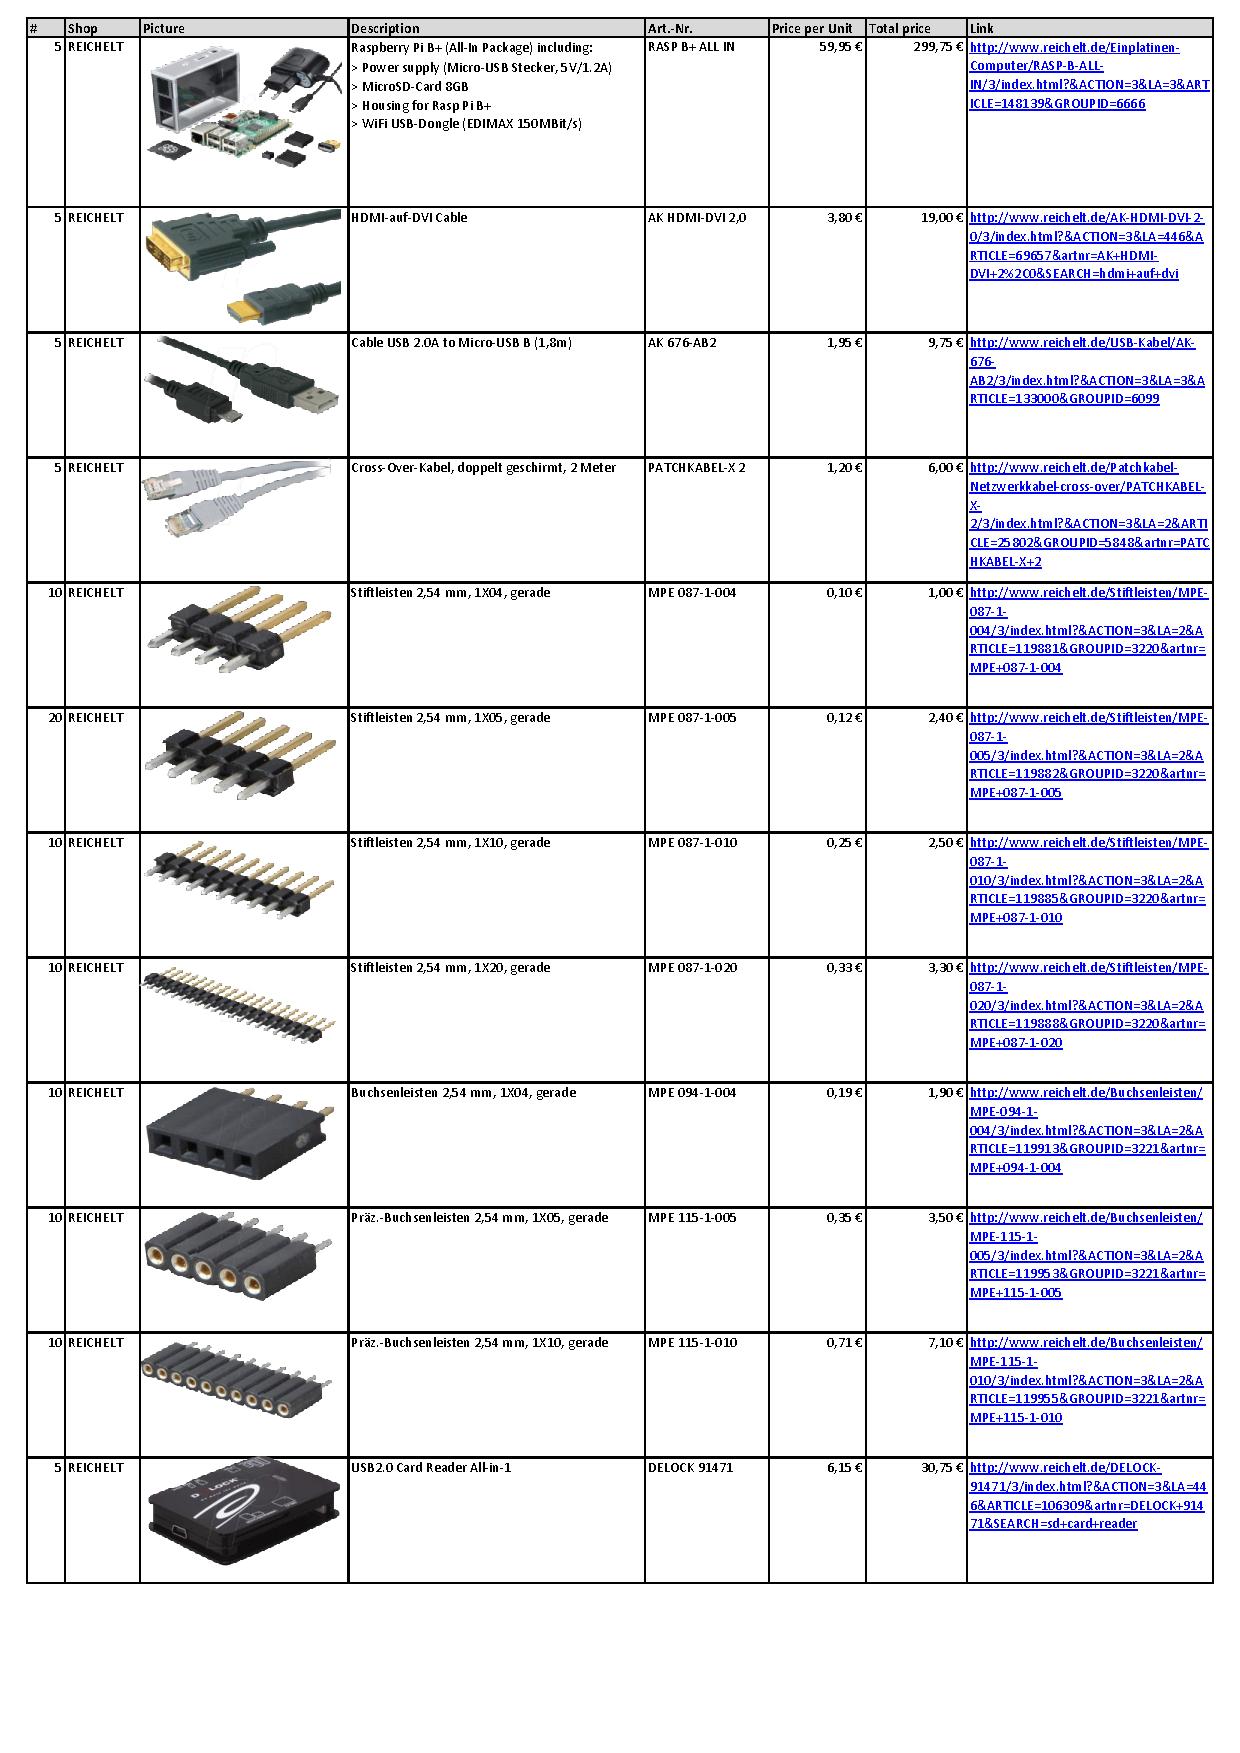
\includegraphics[width=0.90\textwidth,trim=0 80 0 8,clip=true]{fig/ch-rpi-hardware/1_Masterquad2015_BoM}
    \caption{Bill of materials, part 1}
    \label{fig:hardware:BillOfMat:1}
\end{figure}

\begin{figure}[H]
    \centering
    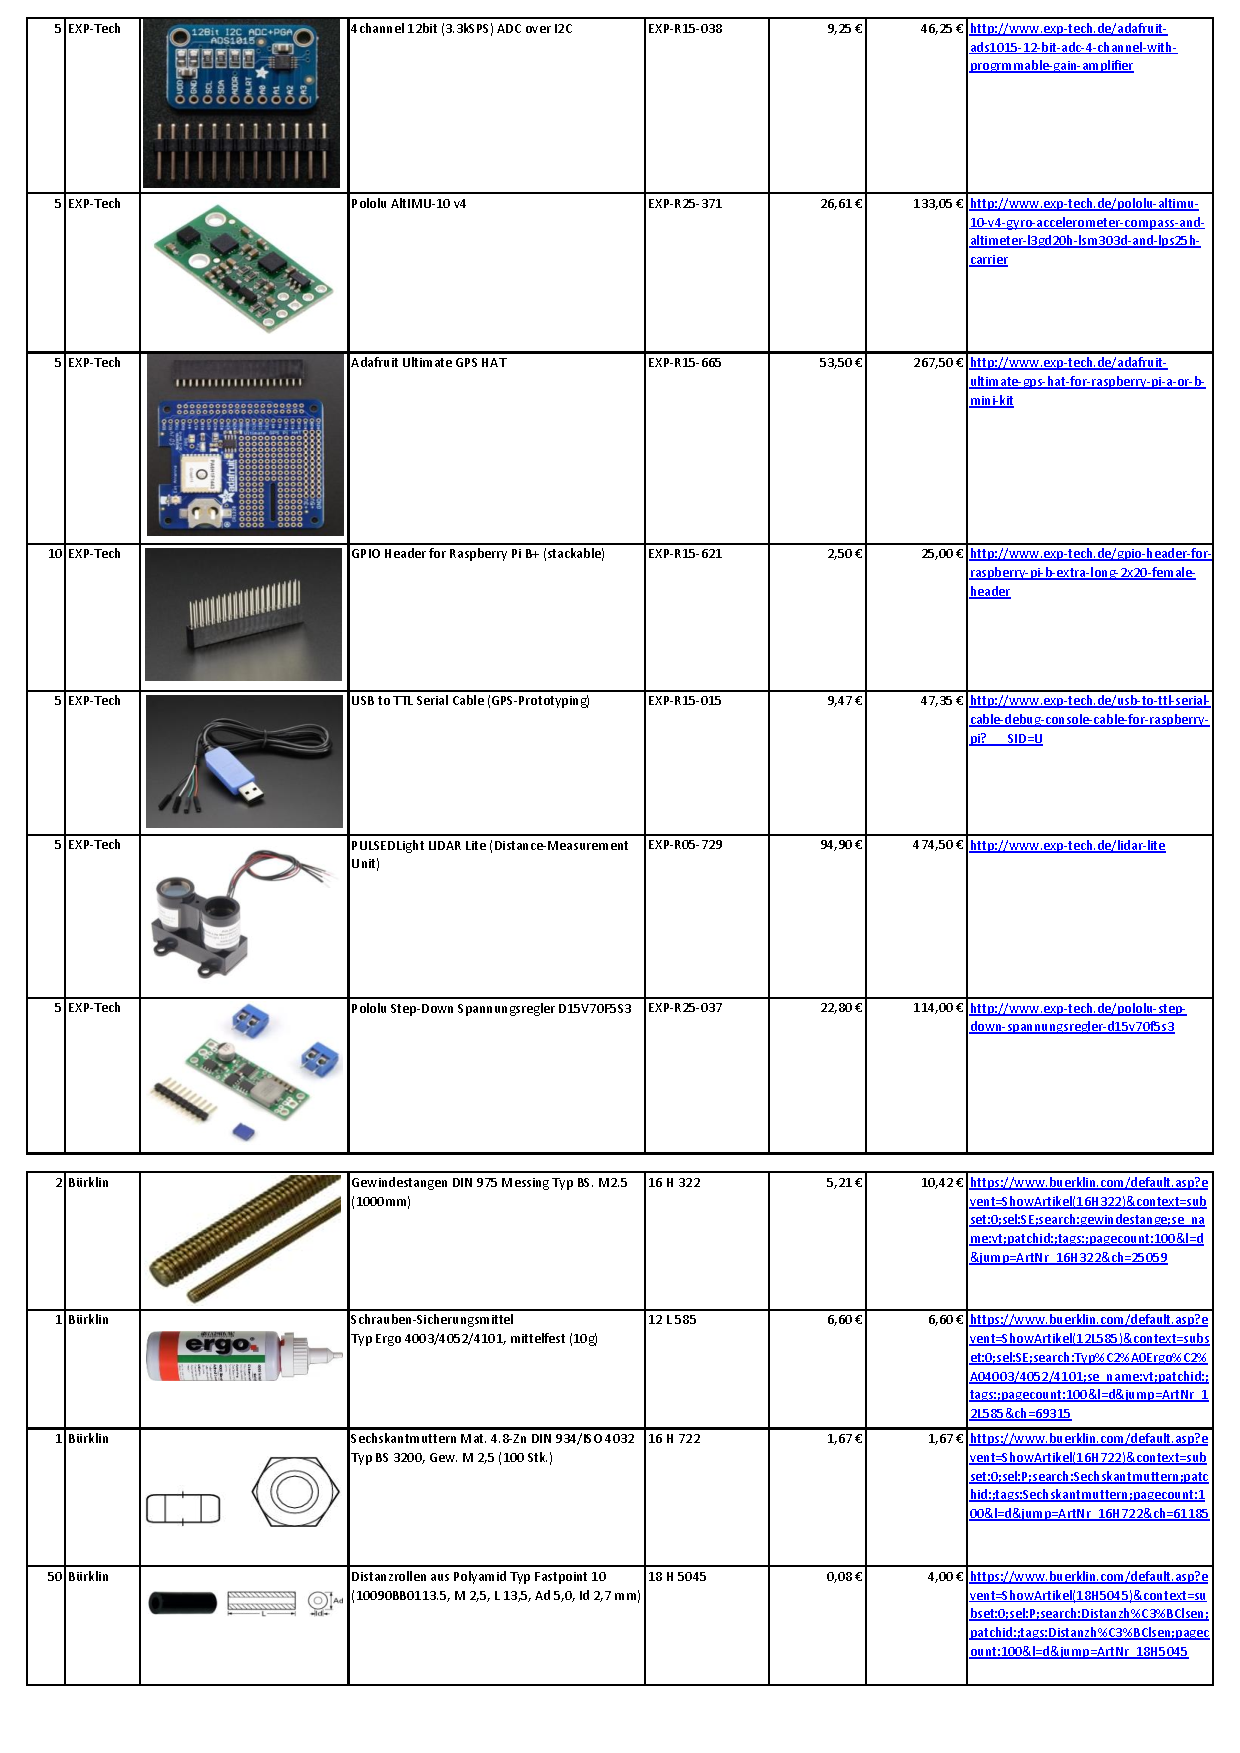
\includegraphics[width=0.97\textwidth,trim=0 31 0 8,clip=true]{fig/ch-rpi-hardware/2_Masterquad2015_BoM}
    \caption{Bill of materials, part 2}
    \label{fig:hardware:BillOfMat:2}
\end{figure}

\begin{figure}[H]
    \centering
    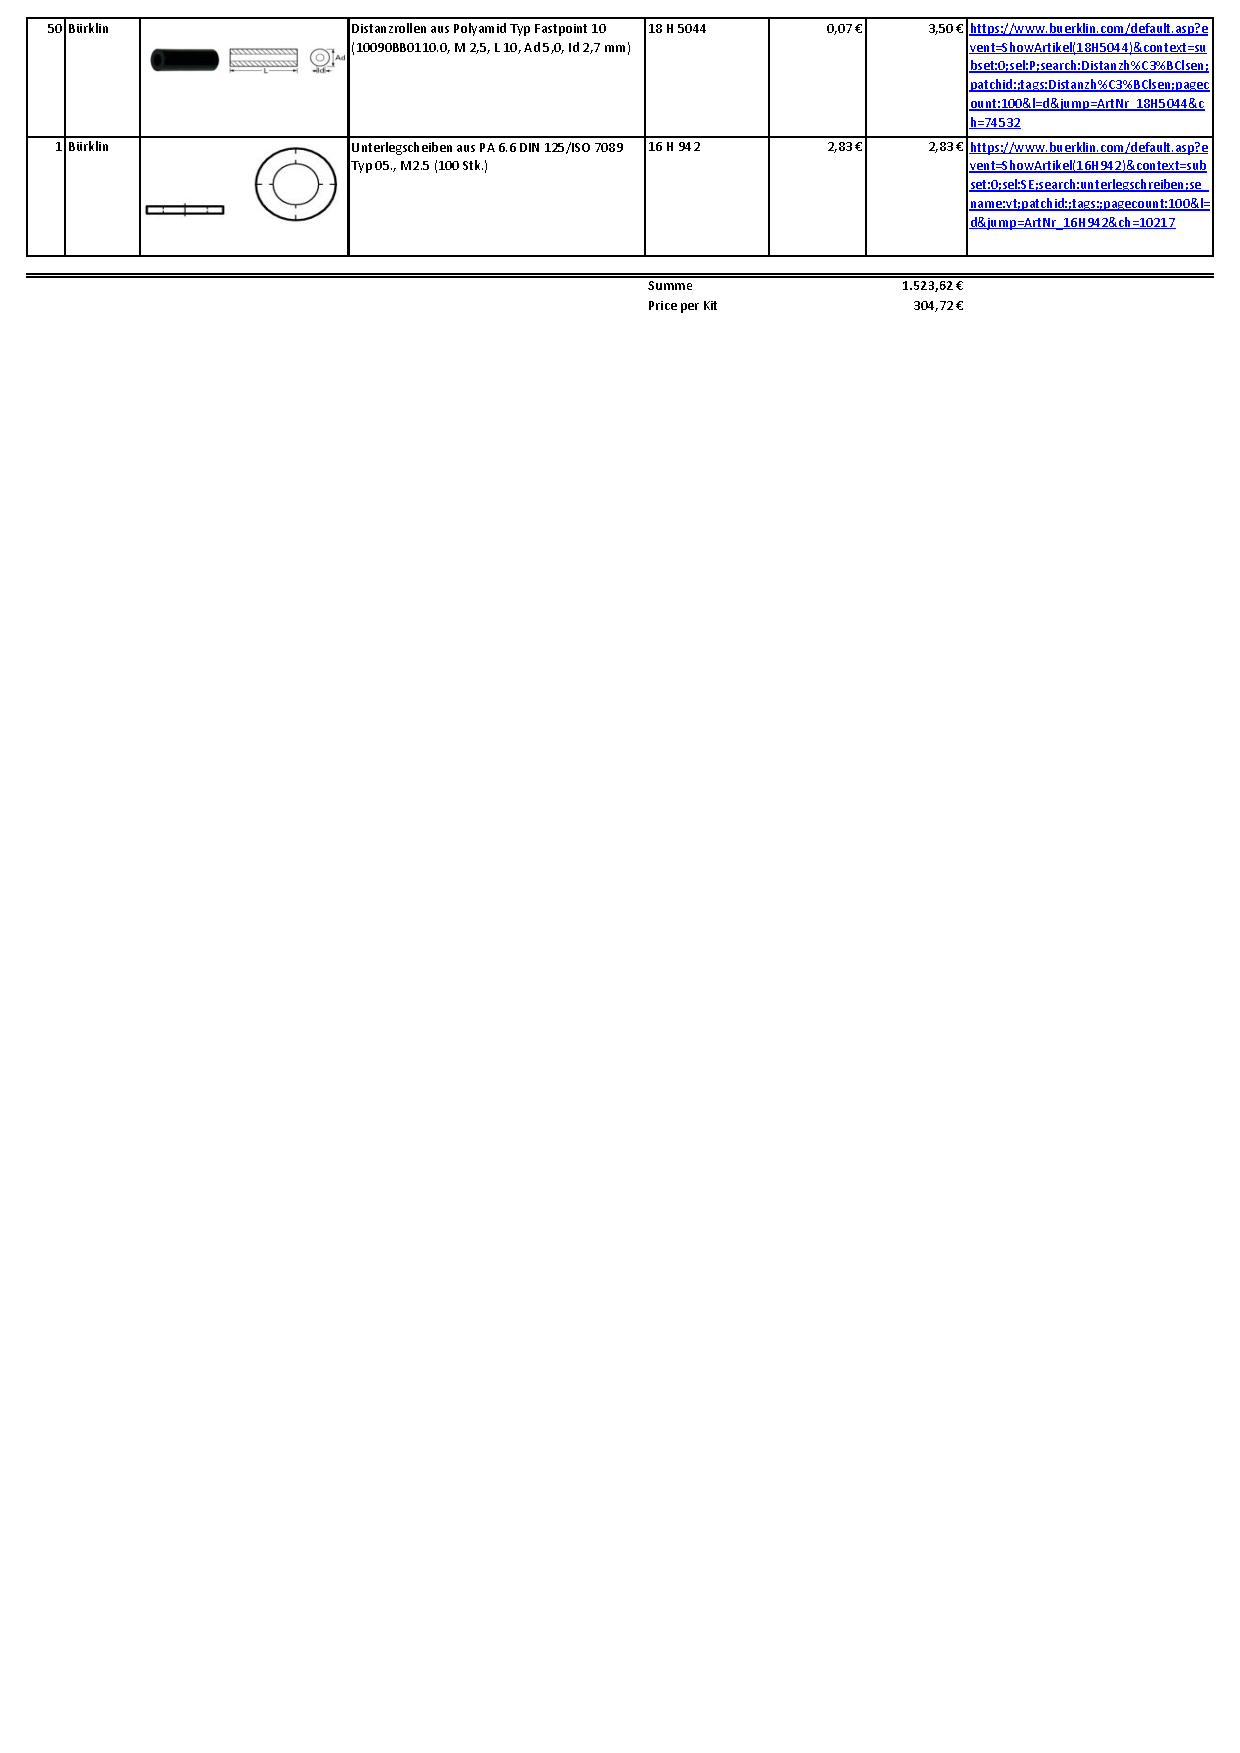
\includegraphics[trim=0 690 0 8,clip=true,width=0.97\textwidth]{fig/ch-rpi-hardware/3_Masterquad2015_BoM}
    \caption{Bill of materials, part 3}
    \label{fig:hardware:BillOfMat:3}
\end{figure}

\chapter{Individual parts}
\label{sec:parts}

\section{Raspberry Pi B+}
\label{sec:goals:rpib}
\begin{figure}[H]
    \centering
    
\includegraphics[width=\textwidth]{fig/ch-rpi-hardware/A4_tech_draw_topview_rpi}
    \caption{Raspberry Pi B+ (topview)}
    \label{fig:parts:rpi_topview}
\end{figure}

\newpage
\section{Adafruit GPS Hat}
\label{sec:goals:gpshat}
\begin{figure}[H]
    \centering
    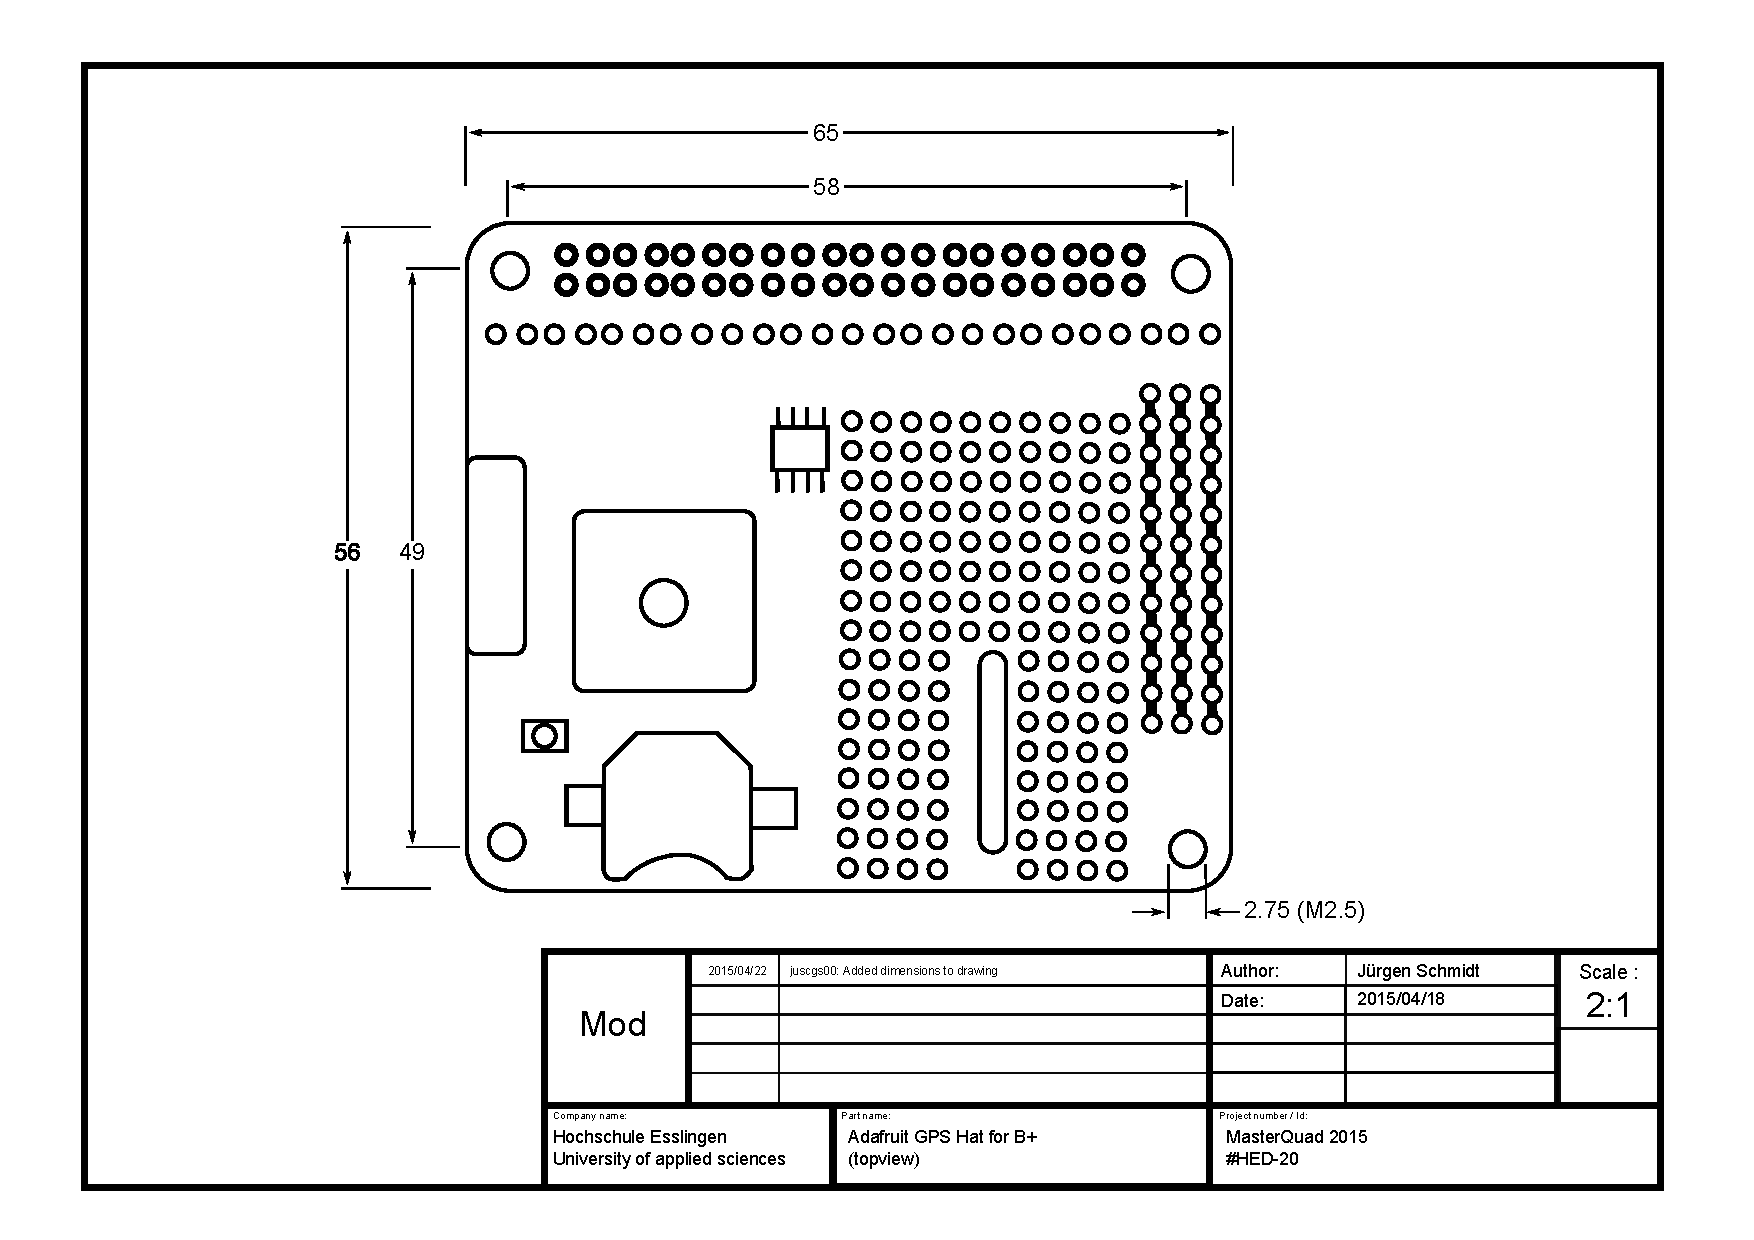
\includegraphics[width=\textwidth]{fig/ch-rpi-hardware/A4_tech_draw_topview_gpshat}
    \caption{Adafruit GPS Hat}
    \label{fig:parts:gps_topview}
\end{figure}

\newpage
\section{Polulu AltIMU v4}
\label{sec:goals:altimu}
\begin{figure}[H]
    \centering
    
\includegraphics[width=\textwidth]{fig/ch-rpi-hardware/A4_tech_draw_topview_imu}
    \caption{Polulu AltIMU v4}
    \label{fig:parts:imu_topview}
\end{figure}

\newpage
\section{Adafruit 12bit ADC over I2C}
\label{sec:goals:adc}
\begin{figure}[H]
    \centering
    
\includegraphics[width=\textwidth]{fig/ch-rpi-hardware/A4_tech_draw_topview_adc}
    \caption{Adafruit 12bit ADC over I2C}
    \label{fig:parts:adc_topview}
\end{figure}

%--------------------------------------------
% Chapter: ASSEMBLY
%--------------------------------------------
\chapter{Assembly}
\label{sec:assemb}

\section{Placing ADC and IMU on GPS Hat}
\label{sec:assemb:sensorsOnHat}
\begin{figure}[H]
    \centering
    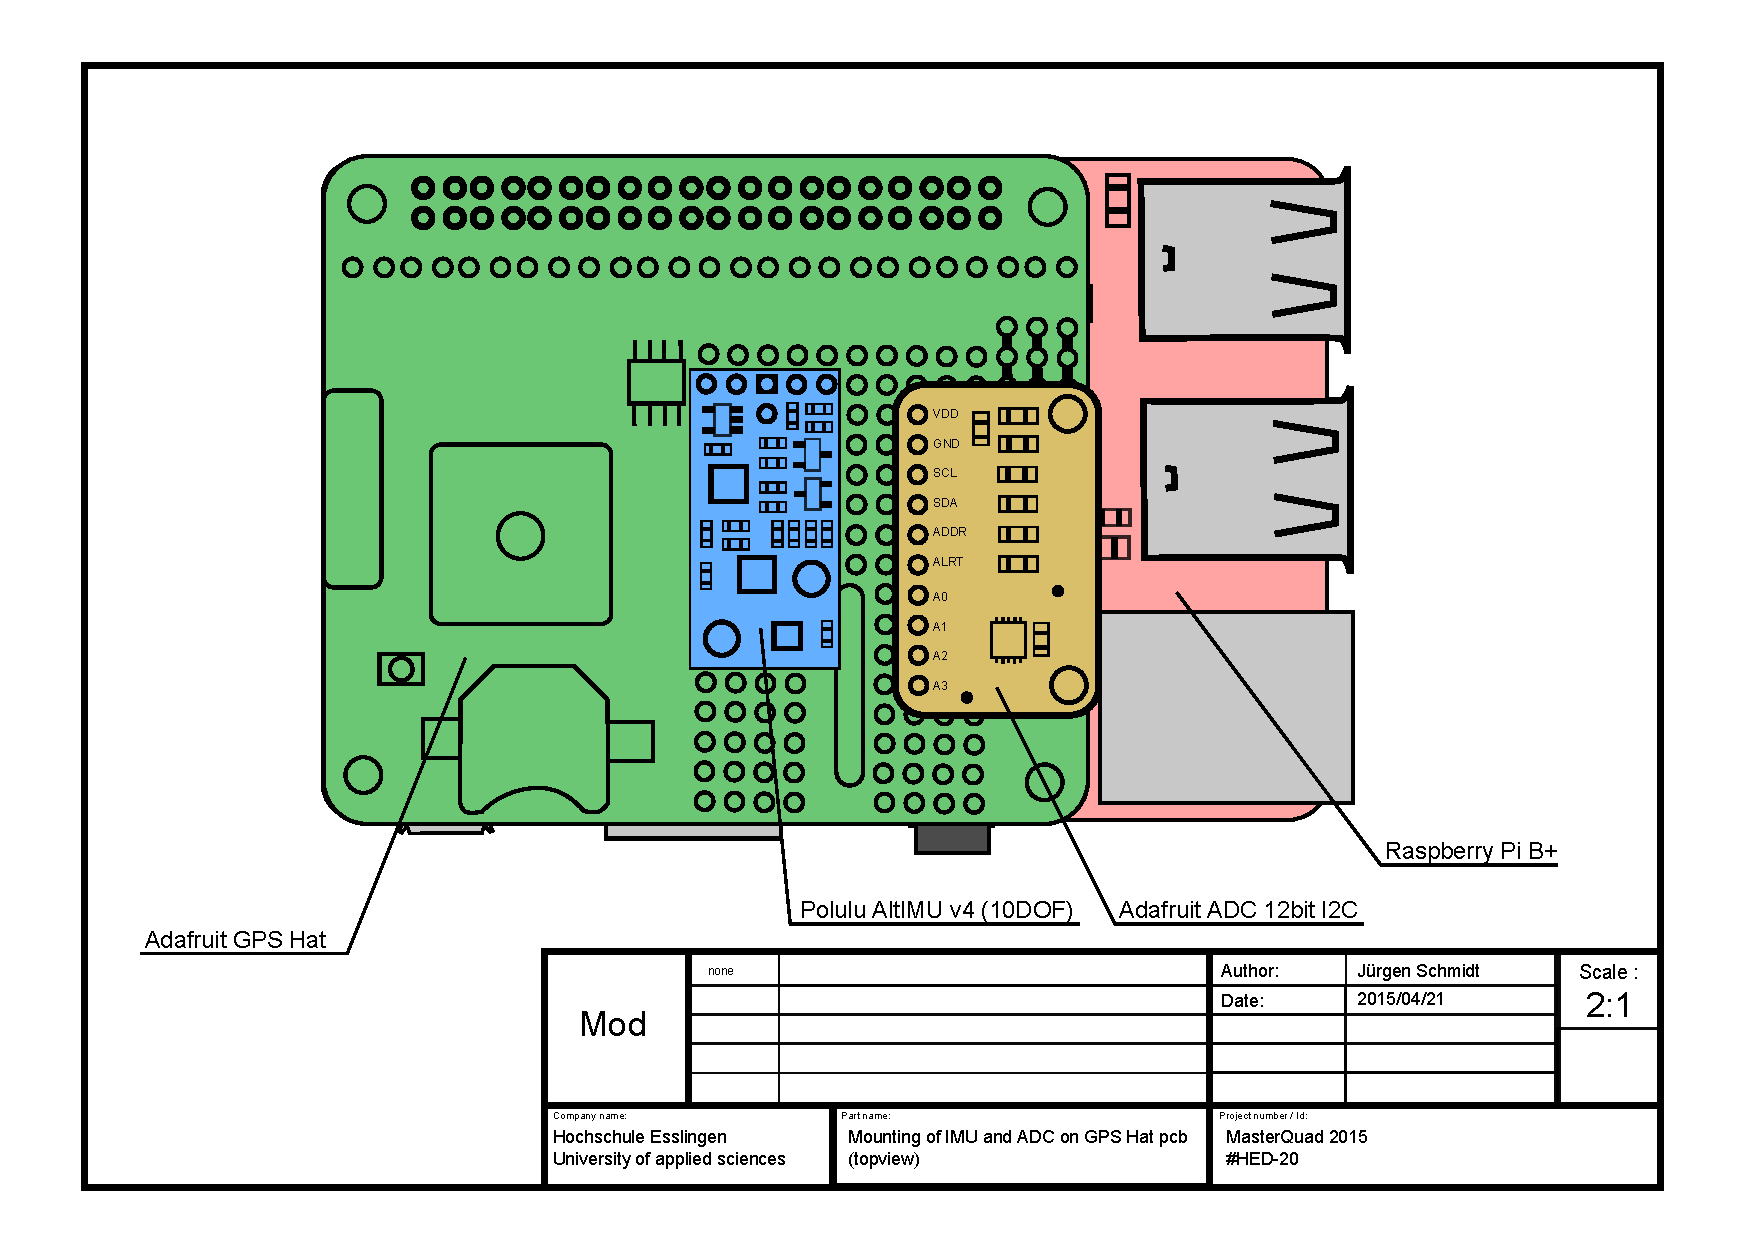
\includegraphics[width=\textwidth]{fig/ch-rpi-hardware/A4_tech_draw_topview_sensor_mountingPositions}
    \caption{Placing ADC and IMU on GPS Hat}
    \label{fig:assemb:sensorMount}
\end{figure}

\section{Wedding of GPS Hat and Raspberry Pi B+}
\label{sec:assemb:wedding}
